% =====================================================================
% Master's Thesis Proposal (Proposta de Dissertacao de Mestrado)
% "Nuanced Facial Expression Synthesis in Generative Models"
% Matheus Levi Rodrigues Aidano -- PPGI / IC-UFAL
%
% Written in ENGLISH. JITH.cls was patched to English (babel + cover/title
% page strings). See NOTES.md for what changed and how to revert.
%
% Build:  latexmk -pdf main.tex          (runs bibtex automatically)
%         makeglossaries main            (once, if the acronym list changes)
% or the explicit sequence:
%         pdflatex main && bibtex main && makeglossaries main \
%           && pdflatex main && pdflatex main
% =====================================================================
\documentclass[12pt,a4paper,oneside]{JITH}
%\documentclass[12pt,a4paper,twoside]{JITH}

% --- Tables ----------------------------------------------------------
\usepackage{booktabs}
\usepackage{tabularx}
\usepackage{array}

% --- Fonts / math ----------------------------------------------------
\usepackage[T1]{fontenc}
\usepackage{amsmath, amsfonts, amssymb, mathtools}
\usepackage{bm}

% --- Figures ---------------------------------------------------------
\usepackage{graphicx}
\graphicspath{{images/}}
\usepackage[caption=false]{subfig}
\usepackage{float}
\usepackage{tikz}
\usetikzlibrary{positioning, arrows.meta, fit, calc, backgrounds}

% --- Text / layout ---------------------------------------------------
\usepackage{indentfirst}
\usepackage{hyperref}
\usepackage{todonotes}          % \todo{...} margin notes -- see NOTES.md
\usepackage{natbib}             % \citep / \citet, apalike style

% glossaries MUST come after hyperref (per its documentation).
\usepackage[acronym, toc, nonumberlist, nogroupskip, nopostdot]{glossaries}
\makeglossaries
\loadglsentries{Cap00/Glossario}

% --- Revision markup (advisor review cycles) -------------------------
% \replace{old}{new} \add{...} \remove{...} \comment{text}{note}
% \highlight{...} \alert{...}
% Use \setreviewsoff before submitting to render the final text clean.
\usepackage{easyReview}
\setreviewson

% =====================================================================
% Macros -- Nuanced Facial Expression Synthesis in Generative Models
%
% HISTORICAL WARNING (kept from the template): the original template's
% macros.tex redefined standard LaTeX commands, notably \S (the section
% symbol) as \mathbb{S}, which broke every "\S\ref{...}" in the text.
% Do NOT redefine single-letter or standard control sequences here.
% =====================================================================

% --- Project nouns ---------------------------------------------------
\newcommand{\genphoto}{\textsc{GenPhoto}}          % Yuan et al. 2024, the base model
\newcommand{\genexpr}{\textsc{GenExpression}}      % this work (rename if desired)
\newcommand{\fineface}{\textsc{FineFace}}          % closest prior art
\newcommand{\mead}{\textsc{MEAD}}                  % training dataset

% --- Notation --------------------------------------------------------
\newcommand{\intensity}{s}                         % commanded intensity scalar
\newcommand{\intensityhat}{\hat{s}}                % detected intensity
\newcommand{\autwelve}{\text{AU12}}                % lip-corner puller
\newcommand{\pearson}{\ensuremath{r}}              % Pearson correlation
\newcommand{\frames}{F}                            % number of frames in a clip

% --- Convenience -----------------------------------------------------
% Placeholder for numbers that still need to be filled in / re-checked.
% Renders visibly so nothing provisional slips into the submitted PDF.
\newcommand{\TBD}{\textcolor{red}{\textbf{[TBD]}}}
% Cross-reference to a lab-notebook entry in docs/experiments/.
\newcommand{\labnote}[1]{\todo[inline, color=blue!12]{lab note: #1}}


\onehalfspacing
\begin{document}
\sloppy

% =====================================================================
\author{Matheus Levi Rodrigues Aidano}
\docTitle{\textbf{Nuanced Facial Expression Synthesis in Generative Models} }

\docType{2}	%%TCC=1; Qualificação Mestrado=2; Dissertação=3; Qualificacao Doutorado=4; Tese=5;

% % % % % % % % % % % % % % % % % % % % % % % % % % % % % %
% % % % % % % % % % % % % % % % % % % % % % % % % % % % % %
%
\orientador{Tiago Figueiredo Vieira}	%%Nome 
\tituloOrientador{Prof. Dr.}
%\coorientador{Ícaro Bezerra Queiroz de Araújo}%%Nome
%\tituloCoorientador{Prof. Dr.}
%
\memberA{Marcelo Costa Oliveira}%%Nome
\filiationA{Prof. Dr., IC-UFAL}%%Titulo, Instituicao
%
\memberB{Thales Miranda de Almeida Vieira}%%Nome
\filiationB{Prof. Dr., IC-UFAL}%%Titulo, Instituicao

% memberC vazio: nao aparece na banca (JITH.cls testa o NOME, nao a filiacao).
% Preencher se houver um terceiro membro.
\memberC{}%%Nome
\filiationC{Prof. Dr., IC-UFAL}%%Titulo, Instituicao

% memberD e memberE: definidos vazios para evitar erro "Undefined control
% sequence" no JITH.cls \folhaDeRosto, que faz \myifnotempty{\@memberD}{...}.
\memberD{}
\filiationD{}
\memberE{}
\filiationE{}

%
% % % % % % % % % % % % % % % % % % % % % % % % % % % % % %
% % % % % % % % % % % % % % % % % % % % % % % % % % % % % %


% Documento escrito em INGLES: o mes deve estar em ingles, pois JITH.cls o
% imprime literalmente no formato "Month DD, YYYY".
\setMonth{June}
\setDate{29}
\setYear{2026}
\setLocation{Maceió, Alagoas}

% % % % % % % % % % % % % % % % % % % % % % % % % % % % % %
% % % % % % % % % % % % % % % % % % % % % % % % % % % % % %
% =====================================================================
\capa
\folhaDeRosto
% \folhaDeAprovacao      % only for the final, signed version

% --- Optional front matter -------------------------------------------
%\agradecimentos
%\epigrafe

% --- Required front matter -------------------------------------------
% Abstract (EN) first because the document is in English; Resumo (PT) is
% kept because Brazilian graduate programs generally require it.
\abstract
\resumo

\listoffigures
\cleardoublepage
\listoftables
\cleardoublepage
\simbolos
\cleardoublepage
\abreviaturas
\cleardoublepage

\tableofcontents
\cleardoublepage

% =====================================================================
\pagenumbering{arabic}

\pagestyle{myheadings}
\renewcommand{\chaptermark}[1]{\markboth{#1}{}}
\renewcommand{\sectionmark}[1]{\markright{#1}}

% =====================================================================
% Chapters
% =====================================================================
\chapter{Introduction}\label{cap:introduction}
\glsresetall

% =====================================================================
% SKELETON. Target: 5--7 pages.
%
% Narrative arc for this chapter, in order:
%   1. Controllable facial expression synthesis matters (applications:
%      affective computing data, avatars, clinical/behavioural stimuli,
%      training data for FER).
%   2. Diffusion models made photorealistic face generation routine, but
%      control over *how much* of an expression is present is still coarse
%      (text prompts are categorical: "smiling" / "not smiling").
%   3. Prior art conditions on continuous AU intensity (\citet{varanka2024fineface})
%      but generates each intensity level as an INDEPENDENT still: nothing
%      binds identity or scene across the levels, and intensity control is
%      reported qualitatively.
%   4. This work reframes expression intensity as a SEQUENCE-level generation
%      parameter: one text prompt plus a per-frame intensity trajectory
%      yields a single temporally coherent clip.
%   5. What was measured so far, honestly (including the negative
%      calibration result) -> forward-reference to Cap05.
%
% Style: impersonal voice, no em-dashes, define every acronym on first use
% via \gls{}. Keep the detailed method out of here (it belongs in Cap04).
% =====================================================================

% =====================================================================
\section{Motivation}\label{sec:motivation}

Controllable synthesis of facial expressions has broad use, and in several of its applications
what matters is not whether a face is smiling but \emph{how much}. Affective-computing and
behavioural studies require stimuli whose expression intensity is varied in a controlled way, and
that intensity is not an incidental parameter of the stimulus. Spontaneous expressions in real
social interaction are frequently of low intensity, whereas conventional stimulus sets portray
emotions only at their peak, a mismatch that motivated the construction of graded-intensity sets
such as the \gls{adfes} Bath Intensity Variations \citep{wingenbach2016adfesbiv}. Its validation
also shows that the axis is behaviourally consequential: recognition accuracy rises monotonically
with intensity, from $56\%$ for low-intensity expressions to $68\%$ at intermediate and $75\%$ at
high intensity. The level at which an expression is rendered therefore determines what a study
using it can measure.

The same axis is a bottleneck for data. Deep \gls{fer} is limited above all by a shortage of
training data \citep{li2022fersurvey}, and intensity-annotated data is the scarcest kind, because
annotating it is slow: coding action-unit intensity under the \gls{facs} \citep{ekman1978facs} can
take an expert more than an hour for a single second of video \citep{tran2017deepcoder}. The
corpora that do carry intensity annotation quantise it coarsely, on a six-point discrete scale in
\gls{disfa} \citep{mavadati2013disfa} or three levels per clip in \gls{mead}
\citep{wang2020mead}. A generator able to render a specified, continuously graded intensity on
demand would relieve both the stimulus and the data problem, provided that the intensity it
renders can be verified properly.

Diffusion models have made photorealistic face generation routine, and text prompts give
convenient high-level control. That control, however, is categorical: a prompt distinguishes
``smiling'' from ``not smiling'', and although language can qualify degree, a phrase such as
``a slight smile'' carries no reproducible mapping onto a measurable intensity. The same words
render differently across prompts, seeds and models, and nothing in the interface allows a smile
to be commanded at a stated fraction of its full extent. What is needed is a numeric axis of
expression intensity on which a diffusion backbone can be conditioned directly, and, for the
sequences that behavioural stimuli and augmentation data require, an axis that varies across the
frames of a single coherent clip rather than across unrelated images.

% =====================================================================
\section{Problem Statement}\label{sec:problem}

% The per-paper analysis of the four closest systems lives in
% Chapter~\ref{cap:related-work} (source material:
% docs/experiments/2026-07-11-related-work-study.md). This section deliberately
% does NOT repeat it. It states the requirements a solution must satisfy, so
% that the contributions of Section~\ref{sec:contributions} and the evaluation
% protocol of Chapter~\ref{cap:method} can be read against them.

The problem is defined by what a solution would have to do. Three requirements follow from the
applications of Section~\ref{sec:motivation}, and a solution must satisfy them at the same time.

\begin{itemize}
    \item \textbf{Numeric Intensity Signal.} The intensity of the expression
    must be specified as a number instead of vague words, and that number must govern each frame
    individually, so that a whole trajectory from neutral to apex can be requested in a single
    instruction.

    \item \textbf{Identity and scene consistency.} If each intensity level is rendered as a separately
    generated image, any difference observed between two levels confounds the change in intensity with a change of identity, pose and scene. For the behavioral stimuli of
    Section~\ref{sec:motivation}, that confound is disqualifying: a response cannot be attributed
    to the intensity of an expression if the face displaying it also changed.

    \item \textbf{Independent Verification.} What was commanded must be checkable against
    what was rendered, and the instrument performing the check must not be the one that produced
    the training labels. Without an independent check the commanded intensity cannot be properly verified, and a model can score well by reproducing the biases of its
    own annotator.
\end{itemize}

No existing system satisfies the three simultaneously. Chapter~\ref{cap:related-work} examines
the closest ones and shows which requirement each relinquishes: expression transfer accepts no
numeric intensity at all; editing methods take a source image as their reference, and so command
a change rather than a value; and action-unit-conditioned generation renders each level as an
independent image.

% =====================================================================
\section{Research Questions}\label{sec:research-questions}

% Keep to two or three. Each must be answerable by an experiment in Cap05
% or by the planned work in Cap06.

\noindent\textbf{Task formulation.} Let a \emph{clip} denote a sequence of $F$ frames
that share one identity and scene. Given a text prompt and a per-frame intensity
trajectory $(s_1,\dots,s_F)$ with each $s_t \in [0,1]$, the objective is to generate a
single clip in which the detected intensity of a given action unit in frame $t$ tracks
$s_t$. This work instantiates the axis with AU12 (lip-corner puller), a proxy for smile
intensity. 

Prior conditional-generation methods instead render each intensity level as an independent image. The three research questions below ask, in turn, whether this trajectory-following is achievable on a frozen \gls{t2v} backbone (RQ1), whether generating the trajectory jointly as one sequence benefits cross-level identity (RQ2), and whether the resulting control is absolute or relative to the commanded trajectory (RQ3). This formulation is restated and made precise
in Chapter~\ref{cap:method}, Section~\ref{sec:method-overview}.

\medskip
\noindent\textbf{RQ1}: Can a scalar expression-intensity axis be injected into a frozen
\gls{t2v} backbone by the same conditioning mechanism that \citet{yuan2024genphoto} apply
to camera parameters, such that the detected AU12 intensity follows a commanded per-frame
trajectory?

\noindent\textbf{RQ2}: Does generating the intensity levels jointly, as a single
sequence, preserve identity across levels better than generating each level as an
independent still?

\noindent\textbf{RQ3}: Is the resulting control absolute, so that a commanded value maps
to a fixed detected intensity, or is it relative to the commanded trajectory, and what
property of the training data determines which?

% =====================================================================
\section{Objectives}\label{sec:objectives}

\subsection{General Objective}\label{subsec:general-objective}

The general objective of this work is to adapt the camera-parameter conditioning mechanism of a
frozen text-to-video diffusion backbone into a facial-expression intensity axis, so that a text
prompt and a per-frame intensity trajectory generate a single identity-consistent clip whose
detected expression intensity follows the command, and to evaluate that control with a protocol
that separately measures trajectory following, absolute calibration, and cross-frame identity.

\subsection{Specific Objectives}\label{subsec:specific-objectives}

\begin{itemize}
    \item Adapt the camera-parameter conditioning mechanism of \citet{yuan2024genphoto} to a facial-expression intensity axis.
    \item Build continuous per-frame AU12 supervision from video (\gls{mead}).
    \item Define an evaluation protocol measuring ramp following, absolute calibration, and cross-frame identity.
    \item Compare head-to-head against the closest prior art under matched prompts.
    \item Characterise the failure modes: calibration, demographic bias, and non-monotonic trajectories.
\end{itemize}

% =====================================================================
\section{Hypotheses}\label{sec:hypotheses}

% Verdicts deliberately kept OUT of this chapter: the hypotheses are stated
% here and adjudicated in Cap05, one subsection each. H3 is refuted there by
% the 2026-07-14 calibration experiment; keeping a refuted hypothesis and
% reporting the refutation is stronger than quietly deleting it.
%   H1 -> Section~\ref{sec:res-ramp}
%   H2 -> Section~\ref{sec:res-headtohead}
%   H3 -> Section~\ref{sec:res-calibration}

Three hypotheses follow from the research questions above. Each is adjudicated against the
measurements of Chapter~\ref{cap:preliminary-results}.

\begin{itemize}
    \item \textbf{H1}: Per-frame scalar conditioning on a frozen backbone yields a detected
    intensity that follows the commanded trajectory.
    \item \textbf{H2}: Joint sequence generation preserves identity across intensity levels
    better than independent per-level generation.
    \item \textbf{H3}: The control is absolute, that is, a commanded value maps to the same
    detected intensity regardless of the surrounding trajectory. Conditioning applied per frame
    and supervised by a per-frame label should in principle fix a mapping from commanded value to
    rendered intensity that is independent of the neighbouring frames.
\end{itemize}

% =====================================================================
\section{Contributions}\label{sec:contributions}

% Claim only what survives the FineFace head-to-head
% (docs/experiments/2026-07-21-fineface-headtohead.md):
%   - ramp-following is a TIE with FineFace, not a win;
%   - FineFace BEATS this work on absolute calibration;
%   - this work wins cross-frame identity, modestly.
% The defensible contribution is therefore the sequence-native formulation
% plus the measurement protocol, NOT better expression control. Any
% "first AU-conditioned generation" phrasing is dead: FineFace (July 2024)
% has primacy. Also avoid "fine-grained" as a headline term, since three of
% the four related papers use it with different meanings.

\noindent This work makes three contributions.

\begin{itemize}
    \item \textbf{C1 (Formulation).} Expression intensity is cast as a \emph{sequence-level}
    generation parameter: one text prompt and one per-frame trajectory yield a single
    identity-consistent clip, whereas the closest prior art \citep{varanka2024fineface} (FineFace)
    produces $N$ independent stills bound only by a shared random seed. Delivered by the
    method overview and conditioning design and evaluated in the head-to-head comparison in Section~\ref{sec:res-headtohead}.
    \item \textbf{C2 (Evaluation protocol).} A protocol that separates three axes commonly
    conflated, namely trajectory-following, absolute calibration, and cross-frame
    identity, and that guards the label/evaluation circularity shared by the closest works
    by scoring with an estimator that produced no training labels. Delivered by
    Section~\ref{sec:method-evaluation} and applied across
    Sections~\ref{sec:res-ramp}--\ref{sec:res-headtohead}.
    \item \textbf{C3 (Empirical characterization).} A quantified commanded-versus-detected
    calibration curve, reported as a single comparable scalar for both this work and FineFace,
    which reports intensity control only qualitatively. The measurements show that ramp-only video
    supervision produces control that is relative to the commanded trajectory rather than absolute. 
    Delivered by Section~\ref{sec:res-calibration}.
\end{itemize}

\noindent Together these establish the contribution as the sequence-native formulation and the evaluation protocol, while also having comparable results with state-of-the-art models.

% =====================================================================
\section{Document Organization}\label{sec:organization}

The remainder of this document is organised as follows. Chapter~\ref{cap:background} introduces
the diffusion, conditioning, temporal-generation, and facial-action-coding machinery on which the
method rests. Chapter~\ref{cap:related-work} positions the work against the closest expression
transfer, editing, and generation systems. Chapter~\ref{cap:method} details the proposed method:
the frozen backbone, the expression conditioning, the training data and setup, and the evaluation
protocol. Chapter~\ref{cap:preliminary-results} reports what has been measured so far. Finally, Chapter~\ref{cap:schedule} lists the completed and remaining
work with the schedule to completion.

\cleardoublepage
% ---------------------------------------------------------------------
\chapter{Background}\label{cap:background}
\glsresetall

% =====================================================================
% SKELETON. Target: 12--18 pages.
%
% Purpose: give the banca exactly the machinery needed to read Cap04, and
% nothing more. Every section here must be load-bearing for the method or
% the evaluation. If a section does not get referenced later, cut it.
%
% Verb tense for literature review: simple present ("X proposes Y").
% =====================================================================

This chapter introduces the machinery needed to read the method and evaluation that follow, and
no more. It proceeds from the generative backbone outward: diffusion models
(Section~\ref{sec:bg-diffusion}) and how they are conditioned (Section~\ref{sec:bg-conditioning});
the temporal mechanism that turns a still-image model into a clip generator
(Section~\ref{sec:bg-temporal}); and the camera-parameter conditioning of Generative Photography
(Section~\ref{sec:bg-genphoto}), whose architecture this work reuses. It then turns to the
expression side: the Facial Action Coding System (Section~\ref{sec:bg-facs}), the tools that
estimate action units (Section~\ref{sec:bg-au-estimation}), the datasets that supply
intensity-graded expressions (Section~\ref{sec:bg-datasets}), and the metrics used to evaluate
control (Section~\ref{sec:bg-metrics}).

% =====================================================================
\section{Diffusion Models}\label{sec:bg-diffusion}

% Forward/reverse process, the noise-prediction objective, and why latent
% space matters for tractability. Keep the derivation minimal: state the
% training objective and move on.
%   \citep{ho2020ddpm}      -- DDPM, forward/reverse formulation
%   \citep{song2021ddim}    -- deterministic sampling, fewer steps
%   \citep{rombach2022ldm}  -- latent diffusion / Stable Diffusion, the backbone here

A diffusion model \citep{ho2020ddpm} defines a forward process that gradually corrupts a data
sample $x_0$ into noise over $T$ steps, $x_t = \sqrt{\bar\alpha_t}\,x_0 +
\sqrt{1-\bar\alpha_t}\,\epsilon$ with $\epsilon\sim\mathcal{N}(0,I)$, and learns to reverse it. In
practice the network $\epsilon_\theta$ is trained to predict the added noise, minimising
$\mathbb{E}_{x_0,\epsilon,t}\,\lVert \epsilon - \epsilon_\theta(x_t,t) \rVert^2$; generation then
denoises from pure noise, and DDIM \citep{song2021ddim} makes this deterministic and possible in
few steps. Operating in pixel space is costly, so latent diffusion \citep{rombach2022ldm} runs the
process in the compressed latent space of a pretrained \gls{vae}, whose encoder maps images to
latents for training and whose decoder maps generated latents back to pixels. Stable Diffusion,
the backbone used in this work, is a latent diffusion model of exactly this form, and every
conditioning mechanism below acts on its denoising network.

% =====================================================================
\section{Conditioning Mechanisms in Text-to-Image Diffusion}\label{sec:bg-conditioning}

% This is the section Cap04 depends on most. Cover, in this order:
%   1. Text conditioning via cross-attention with a CLIP text encoder
%      \citep{radford2021clip}; why it is categorical rather than continuous.
%   2. Classifier-free guidance \citep{ho2022cfg} and its use on a
%      non-text condition.
%   3. Adapter-style injection on a FROZEN backbone: ControlNet
%      \citep{zhang2023controlnet}, IP-Adapter \citep{ye2023ipadapter},
%      LoRA \citep{hu2022lora}. Establish the vocabulary of "decoupled
%      cross-attention" and "zero-initialised merge", both used in Cap04.

Text-to-image diffusion conditions the denoising network on a prompt encoded by a CLIP text
encoder \citep{radford2021clip} and injected through cross-attention layers, in which the image
features attend to the text tokens. This conditioning is effective but \emph{categorical}: a prompt
can say ``smiling'' or ``not smiling'', but expressing \emph{how much} of an expression is present,
on a continuous scale, is beyond what a text token cleanly encodes. Classifier-free guidance
\citep{ho2022cfg} sharpens adherence to any condition by extrapolating between the conditional and
unconditional predictions at sampling time, and applies to non-text conditions as well.

Rather than fine-tuning the whole backbone, control is increasingly added by small modules on a
\emph{frozen} network. ControlNet \citep{zhang2023controlnet} attaches a trainable copy of the
encoder for spatial conditions; IP-Adapter \citep{ye2023ipadapter} adds an image condition through
\emph{decoupled cross-attention}, a parallel attention branch whose output is summed into the text
branch; and \gls{lora} \citep{hu2022lora} injects low-rank updates into existing weight matrices.
Two ideas from this literature recur in Chapter~\ref{cap:method}: decoupled cross-attention, and
the \emph{zero-initialised merge} -- initialising an injected branch to zero so that, before
training, the modified model is identical to the frozen original.

% =====================================================================
\section{Temporal Generation and Motion Modules}\label{sec:bg-temporal}

% The mechanism that makes this work's claim possible: a motion module
% inserted into a 2D UNet turns it into a 3D UNet whose temporal attention
% binds the frames of one clip to a shared identity and scene.
%   \citep{guo2024animatediff} -- AnimateDiff motion module
% Make explicit the point the whole contribution rests on: with temporal
% attention, the frames of a clip are generated JOINTLY, whereas N
% independent stills share only a random seed.

A still-image diffusion model generates each image independently. AnimateDiff
\citep{guo2024animatediff} makes it generate short clips by inserting a \emph{motion module} into
the 2D UNet: temporal-attention layers that let the feature maps of different frames attend to one
another, turning the 2D network into a 3D one. The consequence is central to this work. Because the
frames of a clip are produced \emph{jointly} through temporal attention, they share a single
identity and scene by construction. This is exactly what distinguishes a generated clip from $N$
images sampled independently under a shared random seed: the latter are correlated only through
their starting noise, whereas temporal attention binds them architecturally. The prior art of
Chapter~\ref{cap:related-work} produces the former; this work produces the latter.

% =====================================================================
\section{Parametric Control of Generative Cameras}\label{sec:bg-genphoto}

% The direct antecedent, presented here as background rather than as
% related work because the method in Cap04 reuses its mechanism verbatim.
%   \citep{yuan2024genphoto}
% Cover: the 6-channel physical conditioning layout, the contrastive camera
% learning (\gls{ccl}) text encoding that represents *change between frames*,
% and the zero-initialised merge into temporal attention.

Generative Photography \citep{yuan2024genphoto} adds continuous control over camera parameters --
focal length, bokeh, shutter speed, colour temperature -- to a frozen text-to-video backbone, and
its architecture is reused in Chapter~\ref{cap:method}. A per-frame parameter value is turned into
a six-channel spatial conditioning tensor: three \emph{physical} channels that render the
parameter's effect, and three channels of a text-derived signal encoding the \emph{change} in the
parameter between consecutive frames (the construction its authors term \gls{ccl}). A small
encoder maps this tensor to features that are injected into the backbone's temporal attention
through zero-initialised \emph{merge} weights. This work substitutes an expression-intensity axis
for the camera axis, leaving the six-channel layout, the encoder, and the merge mechanism
unchanged; the substitution is developed in Chapter~\ref{cap:method}.

% =====================================================================
\section{Facial Expression Representation}\label{sec:bg-facs}

% \gls{facs} \citep{ekman1978facs}: anatomically grounded, per-AU, and
% crucially INTENSITY-GRADED, which is what makes a continuous control axis
% meaningful. Justify the choice of AU12 (lip-corner puller) as the single
% axis studied here: unambiguous, high dynamic range, reliably detectable.
% Mention the pre-diffusion lineage of AU-conditioned synthesis
% \citep{pumarola2018ganimation, choi2018stargan}.

The \gls{facs} \citep{ekman1978facs} decomposes any facial expression into \glspl{au}, the
movements of individual muscles or muscle groups, each scored not only as present or absent but on
a graded \emph{intensity} scale. This intensity coding is what makes a continuous control axis
meaningful: an expression is a point on a set of graded axes rather than a discrete label. This
work studies a single such axis, AU12 (the lip-corner puller), the defining action of a smile. AU12
is chosen because it is unambiguous, has a large and visible dynamic range, and is among the more
reliably detected action units, so it is a clean testbed for a continuous axis while the method
itself is not specific to it. Conditioning synthesis on action units predates diffusion: GAN-based
systems such as GANimation \citep{pumarola2018ganimation} and StarGAN \citep{choi2018stargan}
animate or translate expressions from action-unit or categorical labels, but without the
photorealism and text controllability of a diffusion backbone.

% =====================================================================
\section{Automatic Action Unit Estimation}\label{sec:bg-au-estimation}

% These tools are both the source of training labels and the measuring
% instrument, so their properties are part of the method's validity.
%   \citep{cheong2023pyfeat}      -- py-feat, used for labels AND evaluation
%   \citep{lugaresi2019mediapipe} -- MediaPipe blendshapes, independent check
%   \citep{chang2024libreface}    -- LibreFace, used by the prior art
%
% IMPORTANT: introduce the circularity problem HERE (same estimator produces
% labels and scores results), so that Cap04's mitigation reads as a designed
% choice rather than a defensive afterthought. All four related papers share
% this circularity without flagging it; this work flags and mitigates it.

Because no dataset provides per-frame ground-truth action-unit intensities at scale, the
intensities used here are estimated automatically. py-feat \citep{cheong2023pyfeat} predicts a
per-frame AU intensity and is used in this work both to \emph{label} the training data and to
\emph{score} the generated outputs. That double use is a validity concern: when the same estimator
produces the supervision and the metric, a model can score well simply by reproducing its
labeller's biases. The concern is raised here so that the mitigation in Chapter~\ref{cap:method}
reads as a designed choice rather than an afterthought -- a second estimator from a different
family, the face-mesh geometry of MediaPipe \citep{lugaresi2019mediapipe}, which produced none of
the labels, provides an independent check, and agreement between the two is what makes a result
trustworthy. Estimators of this kind, including LibreFace \citep{chang2024libreface}, are also used
by the prior art. All four systems of Chapter~\ref{cap:related-work} label and score with the same
estimator family without noting the circularity; flagging and mitigating it is part of this work's
evaluation.

% =====================================================================
\section{Datasets for Expression Intensity}\label{sec:bg-datasets}

% \gls{mead} \citep{wang2020mead}: multi-view, emotion-labelled, three
% discrete intensity levels, lab conditions. Explain what is extracted here
% that the discrete levels do not give: continuous per-frame AU12 from the
% onset-to-apex ramp of each clip.
% Contrast with the still-image AU datasets used by the prior art:
% DISFA \citep{mavadati2013disfa}, AffectNet \citep{mollahosseini2019affectnet}.
% Note the known consequence of lab-only training data (domain look,
% demographic bias) -- it comes back as a limitation in Cap05.

\gls{mead} \citep{wang2020mead} is a multi-view, emotion-labelled corpus of talking faces recorded
under controlled lighting, with three discrete emotion-intensity levels. The three levels are too
coarse for a continuous axis; what this work extracts instead is a \emph{continuous} per-frame AU12
value along the onset-to-apex ramp of each clip, so that a single clip supplies an ordered sequence
of smoothly increasing intensities. This differs from the still-image action-unit datasets used by
the prior art -- DISFA \citep{mavadati2013disfa}, with manually coded AU intensities, and AffectNet
\citep{mollahosseini2019affectnet}, a large in-the-wild collection -- which provide isolated frames
rather than intensity trajectories. Training on a single lab-recorded corpus carries a known cost
that returns as a limitation in Chapter~\ref{cap:preliminary-results}: the generated faces take on
the dataset's controlled-lighting, frontal appearance, and the model inherits its demographic skew.

% =====================================================================
\section{Evaluation Metrics}\label{sec:bg-metrics}

% Define each metric once, here, then only reference it in Cap04/Cap05.
%   - Pearson r between commanded and detected intensity (ramp following).
%   - \gls{cls}, the control-linearity protocol of \citet{hua2026pixelsmile}:
%     uniformly spaced commanded intensities, correlation against detected.
%   - Face-embedding cosine for identity \citep{deng2019arcface,
%     schroff2015facenet, cao2018vggface2}.
%   - \gls{lpips} \citep{zhang2018lpips} and CLIP-based prompt fidelity.
%   - Note that Pearson r is invariant to scale and offset, which is exactly
%     why an absolute-error metric is also required. This distinction is what
%     separates "follows the ramp" from "is calibrated", and it is the
%     central measurement point of Cap05.

Control is evaluated with a small set of metrics, defined here and only referenced later. Ramp
following is measured by the Pearson correlation $r$ between the commanded per-frame intensity and
the intensity detected in the generated frame. Absolute calibration is measured by the control
linearity score (\gls{cls}) of \citet{hua2026pixelsmile}: uniformly spaced commanded intensities
are correlated against the detected ones. Identity is measured by the cosine similarity of face
embeddings from a recognition network \citep{schroff2015facenet, cao2018vggface2, deng2019arcface};
image quality and prompt fidelity, where reported, use \gls{lpips} \citep{zhang2018lpips} and CLIP
similarity. One property of the correlation is central to Chapter~\ref{cap:preliminary-results}:
Pearson $r$ is invariant to scale and offset, so it rewards a model that \emph{orders and spaces}
the frames correctly even when the detected values are shifted or compressed. Distinguishing
``follows the ramp'' from ``is calibrated'' therefore requires an absolute-error metric -- the
\gls{mse} of the detected value against the commanded one -- alongside the correlation.

\cleardoublepage
% ---------------------------------------------------------------------
\chapter{Related Work}\label{cap:related-work}
\glsresetall

% =====================================================================
% SKELETON. Target: 8--12 pages.
%
% Source material: docs/experiments/2026-07-11-related-work-study.md holds
% full per-paper analyses (method, data, metrics, headline numbers with
% section references) from complete reads of the four PDFs in related_work/.
% Pull the prose from there; do not re-derive it.
%
% Organise BY TASK FORMULATION, not chronologically. The whole point of the
% chapter is to show that the four closest systems solve three different
% problems, and that none solves the one posed in Chapter~\ref{cap:introduction}.
% =====================================================================

\todo[inline]{Opening paragraph: the three task formulations (transfer, editing, generation) and where this work sits.}

% =====================================================================
\section{Expression Transfer from an Exemplar}\label{sec:rw-transfer}

% \citet{jiang2024emojidiff}: control signal is an RGB exemplar image
% (masked face, CLIP-encoded) injected via IP-Adapter-style decoupled
% cross-attention into frozen SD1.5; identity from a reference photo;
% ArcFace identity loss on one-step decodes.
% Relation: adjacent, not competing. It cannot accept "smile = 0.5" as
% input; a user must supply an exemplar per intensity level.
% Their Sec. 1 critique of signal-conditioned methods (detail loss,
% dependence on third-party detector accuracy) applies to this work and
% should be acknowledged and answered in Cap04.

\todo[inline]{EmojiDiff: mechanism, why exemplar conditioning is not a numeric control axis.}

% =====================================================================
\section{Expression Editing of a Source Image}\label{sec:rw-editing}

\subsection{Action-Unit Conditioned Editing}\label{subsec:rw-magicface}

% \citet{wei2025magicface}: 12-dim AU *variation* vector (target minus
% source), injected through a linear layer added to the time embedding;
% FULL fine-tune of the denoising UNet plus a UNet-copy ID encoder;
% AU dropout plus CFG on the AU condition.
% Relation: closest in control semantics (continuous AU intensity on SD),
% but editing rather than generation, relative rather than absolute targets
% (requires source-AU estimation at inference), no temporal mechanism, and
% far more trainable parameters.
% Their lab-vs-wild ablation predicts this work's lab-domain artifacts.

\todo[inline]{MagicFace: relative AU vectors, full fine-tune, and what "relative" costs at inference.}

\subsection{Intensity as a Text-Embedding Direction}\label{subsec:rw-pixelsmile}

% \citet{hua2026pixelsmile}: intensity alpha scales a text-embedding
% direction on Qwen-Image-Edit with LoRA; source of the CLS protocol
% adopted in Cap04.
% Two points must be made:
%   1. Their zero-shot row (no training, text-embedding interpolation alone)
%      already achieves substantial linearity. This is the "why not just
%      prompt it?" objection and it must be answered, not ignored -- hence
%      the prompt-engineering baseline planned in Cap06.
%   2. Their negative MEAD result does NOT transfer: they mapped MEAD's
%      three discrete levels to {0.5, 0.75, 1.0}, discarding the continuous
%      per-frame signal this work extracts.

\todo[inline]{PixelSmile: the CLS protocol, the zero-shot baseline objection, why their MEAD result does not transfer.}

% =====================================================================
\section{Action-Unit Conditioned Generation}\label{sec:rw-fineface}

% THE PRIOR ART. State this plainly and early: \citet{varanka2024fineface}
% (July 2024) generates faces from text conditioned on a continuous 12-dim
% AU intensity vector, with no source image, using an adapter on a frozen
% backbone plus CFG on the AU condition, and demonstrates out-of-range
% extrapolation. Its control is BROADER than this work's single AU12 axis.
% Any claim of primacy for "AU-conditioned generation" is therefore
% unavailable and must not appear anywhere in the text.
%
% What it does not do, and this is the opening this work occupies:
%   - its intensity sweep is N INDEPENDENT stills, sharing only a seed;
%     nothing binds identity across levels architecturally;
%   - it reports NO face-identity metric at all;
%   - intensity control is shown qualitatively only, with the authors
%     conceding the scale is nonlinear; there is no commanded-vs-detected
%     correlation anywhere.

\todo[inline]{FineFace: present as prior art, precisely delimit what it leaves open.}

% =====================================================================
\section{Positioning}\label{sec:rw-positioning}

% The table below is transcribed from the comparison in
% docs/experiments/2026-07-11-related-work-study.md. Verify each cell
% against the papers before submitting, and keep the "Ours" column honest:
% the FineFace head-to-head (2026-07-21) showed ramp-following is a TIE and
% that FineFace WINS absolute calibration. The differentiator is the
% sequence-native formulation and the measurement protocol.

\begin{table}[H]
    \centering
    \caption{Positioning of this work against the closest systems.}
    \label{tab:positioning}
    \footnotesize
    \begin{tabularx}{\textwidth}{@{}l>{\raggedright\arraybackslash}X>{\raggedright\arraybackslash}X>{\raggedright\arraybackslash}X@{}}
        \toprule
        Axis & MagicFace / PixelSmile & FineFace & This work \\
        \midrule
        Task              & editing a source image      & generation, independent stills   & generation, one coherent clip \\
        Control input     & relative AU vector / unitless $\alpha$ & absolute 12-AU vector   & per-frame AU12 trajectory \\
        Source image       & required                   & not required                     & not required \\
        Identity across levels & loss term (single image) & no mechanism, no metric        & temporal attention (measured) \\
        Intensity reported as & aggregate error / VLM-judged & qualitative sweeps          & correlation + absolute error \\
        Label/eval circularity & unflagged               & unflagged                        & flagged and mitigated \\
        \bottomrule
    \end{tabularx}\\[4pt]
    {\footnotesize Source: prepared by the author.}
\end{table}

\todo[inline]{Closing paragraph: state the gap this work fills, in one sentence, and forward-reference Cap04.}

\cleardoublepage
% ---------------------------------------------------------------------
\chapter{Proposed Method}\label{cap:method}
\glsresetall

% =====================================================================
% SKELETON. Target: 12--16 pages. The core chapter of the proposal.
%
% Ground truth for every claim here: docs/status.md (living state) and the
% dated entries in docs/experiments/. Code paths are listed in the file map
% at the end of docs/status.md. If a number appears in this chapter, it must
% trace to a lab-notebook entry.
%
% Rule for a PROPOSAL: separate clearly what is BUILT AND VERIFIED from what
% is PLANNED. The banca will ask. Cap06 holds the schedule for the planned
% part; this chapter should mark it inline.
% =====================================================================

\todo[inline]{Opening paragraph: one-sentence statement of the method, then the chapter roadmap.}

% =====================================================================
\section{Overview}\label{sec:method-overview}

% Reframe the task formally: given a text prompt p and a per-frame intensity
% trajectory (s_1, ..., s_F), generate ONE clip of F frames sharing identity
% and scene, in which the detected AU12 intensity of frame t tracks s_t.
% Contrast in one sentence with the prior-art formulation (F independent
% samples), since that contrast is the contribution.
%
% A system figure belongs here. Suggested content: text prompt and intensity
% list on the left; expression encoder producing the conditioning tensor;
% frozen SD1.5 UNet plus AnimateDiff motion module in the middle; the
% zero-initialised merge into temporal attention highlighted; output clip on
% the right; frozen vs trainable components colour-coded. Draw with TikZ
% (already loaded) and save nothing to images/ unless it is a raster.

\todo[inline]{Formal task statement + system figure. Colour-code frozen vs trainable.}

% =====================================================================
\section{Backbone and Trainable Components}\label{sec:method-backbone}

% Be exact and verifiable about what trains and what does not:
%   Frozen: SD1.5 UNet, VAE, CLIP text encoder, AnimateDiff motion module.
%   Trainable: the expression encoder and the attention merge weights.
% Give the trainable parameter count and contrast it with the fully
% fine-tuned prior art (see the comparison in the related-work study note).
% State the compute honestly: a single RTX 3090, 100k steps. This is a
% strength of the proposal, not something to hide.

\todo[inline]{Table of frozen vs trainable modules with parameter counts.}

% =====================================================================
\section{Expression Conditioning}\label{sec:method-conditioning}

\subsection{Intensity Embedding}\label{subsec:method-embedding}

% The scalar intensity is broadcast into the 6-channel conditioning layout
% inherited from \citet{yuan2024genphoto} (cin: 384), so the mechanism is
% unchanged from the camera-parameter original. Explain what replaces the
% physical channels (blur kernel, crop mask) and why a scalar broadcast is
% the right first formulation.
% Name it as "Option A" if that vocabulary is kept from docs/plan.md, and
% state the alternative (landmark flow, multi-AU vector) as future work.

\todo[inline]{Describe create\_intensity\_embedding: scalar to 6-channel broadcast, dimensions.}

\subsection{Change Encoding in the Text Branch}\label{subsec:method-ccl}

% The \gls{ccl} text encoding represents the direction and magnitude of
% change BETWEEN consecutive frames, which is meaningless in a single-image
% setting and is therefore genuinely specific to this formulation. Show the
% prompt template ("<smile intensity: ...>") and how it differs from
% GenPhoto's camera phrasing.

\todo[inline]{CCL adaptation: prompt template and the between-frames semantics.}

\subsection{Injection into Temporal Attention}\label{subsec:method-merge}

% The merge weights are zero-initialised, which has a useful consequence
% worth stating explicitly: with no adaptor checkpoint loaded, the model is
% bit-identical to the unmodified backbone. That is what makes the ablation
% baseline provably fair (verified 2026-07-09), and it is a small but real
% methodological point.

\todo[inline]{Merge mechanism + the zero-init equals frozen-backbone equivalence argument.}

% =====================================================================
\section{Training Data}\label{sec:method-data}

% MEAD front-view "happy" clips \citep{wang2020mead}; MediaPipe crops;
% continuous per-frame AU12 labels from py-feat \citep{cheong2023pyfeat};
% train/validation split sizes from docs/status.md.
% State the two known data limitations here rather than burying them:
%   1. clips are onset-to-apex RAMPS only, which is the root cause of the
%      calibration result in Cap05;
%   2. MEAD "happy" clips carry high AU12 even at low labelled levels.

\todo[inline]{Preprocessing pipeline, split sizes, label extraction, and the ramp-only property of the data.}

% =====================================================================
\section{Training Setup}\label{sec:method-training}

\todo[inline]{Objective, optimiser, schedule, batch/accumulation, steps, hardware, checkpointing.}

% =====================================================================
\section{Evaluation Protocol}\label{sec:method-evaluation}

% This section is a contribution in its own right, because none of the four
% closest papers measures all three axes. Present it as three separate
% questions with separate instruments.

\subsection{Trajectory Following}\label{subsec:eval-ramp}

% Pearson r between the commanded per-frame intensity and the AU12 intensity
% detected in the generated frame. Report the prompt bank size and the number
% of seeds so the protocol is reproducible.

\todo[inline]{Ramp-following protocol: prompt bank, seeds, correlation computation.}

\subsection{Absolute Calibration}\label{subsec:eval-calibration}

% The measurement that separates "follows a ramp" from "is calibrated":
% hold the commanded value CONSTANT across the clip and vary it between
% clips; a calibrated model changes its output, an ordinal one does not.
% Adopt the \gls{cls} protocol of \citet{hua2026pixelsmile} for
% comparability, plus an absolute-error complement, because Pearson r is
% invariant to scale and offset (Section~\ref{sec:bg-metrics}).

\todo[inline]{Constant-list and permuted-list designs; CLS plus absolute error.}

\subsection{Identity Consistency}\label{subsec:eval-identity}

% Frame-to-frame face-embedding cosine within a generated clip
% \citep{schroff2015facenet, cao2018vggface2}, and the same measurement
% across the independent stills of the baseline. Report the adjacent-frame
% minimum, not just the mean, since the worst transition is what a viewer
% notices. Multi-model averaging (adding ArcFace \citep{deng2019arcface})
% is planned; see Cap06.

\todo[inline]{Identity protocol: embedding model(s), adjacent-frame minimum, baseline treatment.}

\subsection{Guarding Against Label--Evaluation Circularity}\label{subsec:eval-circularity}

% The honest statement of a real threat: py-feat produces the training
% labels AND the primary metric. Mitigation is a second estimator from a
% different family (MediaPipe mouth-corner geometry) that touched no labels.
% Worth stating that all four studied papers share this circularity without
% flagging it, so doing so is an evaluation contribution rather than an
% admission of weakness.

\todo[inline]{State the circularity, the independent-detector mitigation, and its limits.}

% =====================================================================
\section{Baselines}\label{sec:method-baselines}

\begin{itemize}
    \item \textbf{Frozen backbone.} Same seed, no expression conditioning; provably identical to the unmodified backbone by the zero-init argument of Section~\ref{subsec:method-merge}. Isolates the effect of the trained adaptor.
    \item \textbf{Prior art, matched prompts.} \citet{varanka2024fineface} run as independent stills over the same prompts and intensity levels. This is the comparison that isolates the sequence-native claim.
    \item \textbf{Prompt engineering.} Graded textual descriptions of smile intensity on the unmodified backbone, answering the "why not just prompt it?" objection raised by the zero-shot result of \citet{hua2026pixelsmile}. \todo[inline]{Planned, not yet run: see Cap06.}
\end{itemize}

% Reproducibility note worth one short paragraph: inference is seed-locked
% (re-seeded immediately before sampling), so the same seed and config give
% bit-identical outputs and ablations differing only in construction-time RNG
% draws remain comparable.

\todo[inline]{Add the seed-control reproducibility paragraph.}

\cleardoublepage
% ---------------------------------------------------------------------
\chapter{Preliminary Results}\label{cap:preliminary-results}
\glsresetall

% =====================================================================
% SKELETON. Target: 10--14 pages.
%
% The tables below are PRE-FILLED from docs/status.md as of 2026-08-06, with
% the originating lab note given in each caption. Cross-check every number
% against its dated entry in docs/experiments/ before submitting; those files
% are append-only and authoritative, docs/status.md is a living summary.
%
% Reporting principle for this chapter: the negative calibration result and
% the tie with the prior art are REPORTED, not softened. They are what make
% the contribution claim in Chapter~\ref{cap:introduction} defensible, and a
% banca that finds them by asking will trust the rest of the document less.
% =====================================================================

This chapter reports what has been measured on the trained model to date. Each section
isolates one property with its own instrument: trajectory following
(Section~\ref{sec:res-ramp}), identity consistency across the trajectory
(Section~\ref{sec:res-identity}), absolute calibration (Section~\ref{sec:res-calibration}),
the emergence of the capability over training (Section~\ref{sec:res-dose}), a head-to-head
against the closest prior art (Section~\ref{sec:res-headtohead}), and the whole-face response
to the single axis (Section~\ref{sec:res-coactivation}). The negative calibration result and
the tie with the prior art are reported plainly rather than softened: they are what make the
contribution claim of Chapter~\ref{cap:introduction} defensible. Every number traces to the
dated laboratory note cited in its caption.

% =====================================================================
\section{Experimental Setup}\label{sec:res-setup}

% Checkpoint (100k steps, single RTX 3090), prompt bank size, seeds,
% frames per clip, intensity lists used. Point to the batch-eval harness so
% the numbers are reproducible.

All numbers below come from the released 100k-step checkpoint
(Section~\ref{sec:method-training}), generated on a single RTX~3090. Unless a table states
otherwise, evaluation uses the bank of 40 text prompts, three seeds ($42,43,44$), and
five-frame clips at $256\times384$, decoded at 25 denoising steps with classifier-free
guidance scale $8.0$. The ascending ramp commands the intensity list $(0,0.25,0.5,0.75,1.0)$;
the constant-list and permuted-list designs of Section~\ref{sec:method-evaluation} supply the
calibration and non-monotonic probes. Generation and scoring run through the
batch-evaluation harness, so every reported figure is reproducible from the same seeds and
configuration.

% =====================================================================
\section{Trajectory Following}\label{sec:res-ramp}

% Headline: control over the trajectory is real and robust at scale, and it
% is confirmed by an estimator that produced none of the training labels.
% The descending-ramp reversal near -1 is strong evidence that the model
% responds to the conditioning signal rather than to a fixed temporal prior.

\begin{table}[H]
    \centering
    \caption{Trajectory following, measured as Pearson correlation $r$ between commanded and detected AU12 intensity, with the per-condition sample size $n$.}
    \label{tab:res-ramp}
    \begin{tabular}{@{}lccc@{}}
        \toprule
        Condition & $n$ & py-feat AU12 $r$ & MediaPipe proxy $r$ \\
        \midrule
        Trained adaptor, ascending ramp  & $120$ & $0.774 \pm 0.212$ & $0.829 \pm 0.230$ \\
        Frozen backbone baseline         & $120$ & $-0.05 \pm 0.64$  & $-0.02 \pm 0.66$ \\
        Trained adaptor, descending ramp & $1$   & $-0.98$           & not measured \\
        Trained adaptor, permuted list   & $90$  & $0.385 \pm 0.505$ & $0.46 \pm 0.45$ \\
        \bottomrule
    \end{tabular}\\[4pt]
    {\footnotesize Source: prepared by the author. Lab notes 2026-07-08 and 2026-07-14. The baseline MediaPipe proxy is computed on only the 44/120 clips with a valid measurement, which flatters it; the descending-ramp MediaPipe proxy was not measured (that run predates MediaPipe scoring).}
\end{table}

Table~\ref{tab:res-ramp} establishes that trajectory following is real and robust at scale.
On the ascending ramp the trained adaptor reaches $r=0.774\pm0.212$ (median $0.86$, with
$87\%$ of clips above $0.5$), against a frozen-backbone baseline indistinguishable from zero.
The result is corroborated by the MediaPipe proxy ($r=0.829$), an estimator that produced none
of the training labels, so the effect is not an artefact of the py-feat pipeline. The
descending-ramp reversal to $r=-0.98$ shows the model tracks the commanded signal rather than a
fixed temporal prior. The permuted-list drop to $r=0.385\pm0.505$ is a scope statement rather
than a failure: the conditioning is genuinely per-frame, but the temporal prior resists
non-monotonic trajectories, for which the ramp-only training data offers no support.

% Interpretation point worth making explicitly: the permuted-list result
% (0.385) shows the conditioning is genuinely per-frame, but that the
% temporal prior resists non-monotonic trajectories, for which the training
% data contains no support. This is a scope statement, not a failure.

% =====================================================================
\section{Identity Consistency}\label{sec:res-identity}

% The measurement that isolates the sequence-native claim. Note the
% qualitative asymmetry that matters as much as the number: the baseline's
% faces were undetectable in 57% of samples, so its 0.85 is computed on the
% easier remainder and flatters it.

\begin{table}[H]
    \centering
    \caption{Frame-to-frame face-embedding cosine similarity within a generated clip. The adjacent-frame minimum, the worst single transition, is the quantity the head-to-head comparison turns on.}
    \label{tab:res-identity}
    \begin{tabular}{@{}lccc@{}}
        \toprule
        Condition & Mean cosine & Adjacent-frame min. & Face detected \\
        \midrule
        Trained adaptor          & $0.92 \pm 0.05$ & $0.877 \pm 0.086$ & $120/120$ \\
        Frozen backbone baseline & $0.85$          & $0.794 \pm 0.152$ & $43\%$ \\
        \bottomrule
    \end{tabular}\\[4pt]
    {\footnotesize Source: prepared by the author. Lab note 2026-07-14, facenet-VGGFace2 embeddings. The baseline's faces were undetectable in 57\% of samples, so its cosines are computed on the easier remainder.}
\end{table}

Table~\ref{tab:res-identity} isolates the sequence-native claim. Within a generated clip the
trained adaptor holds a frame-to-frame identity cosine of $0.92\pm0.05$ and, more tellingly, an
adjacent-frame minimum of $0.877\pm0.086$ against the baseline's $0.794\pm0.152$; the
adjacent-frame minimum is reported because the worst transition is the one a viewer notices, and
it is the quantity the head-to-head comparison turns on. The comparison is not quite symmetric:
the baseline's faces were undetectable in $57\%$ of samples, so its cosines are computed on the
easier detectable remainder and are flattered. Identity is measured here with a single embedding
network (facenet-VGGFace2); multi-model averaging with an ArcFace embedding is scheduled as
proposed work in Chapter~\ref{cap:schedule}.

% =====================================================================
\section{Absolute Calibration}\label{sec:res-calibration}

% NEGATIVE RESULT. Report it plainly and diagnose it.
%
% Finding: holding the commanded value constant across a clip and varying it
% between clips produces almost no change in detected intensity
% (\gls{cls} = 0.07; detected AU12 flat near 0.85 for every commanded level
% at or above 0.1). The same commanded value of 0.0 renders as 0.54 inside a
% ramp and 0.79 in a constant clip.
%
% Consequence: the control is RELATIVE and contextual, not absolute. The
% conditioning commands a trajectory, not a value.
%
% Root cause: the training clips are onset-to-apex ramps only
% (Section~\ref{sec:method-data}), so the model never observed a constant
% intensity trajectory.
%
% This refutes H3 from Section~\ref{sec:hypotheses}. Say so in those words.

The calibration measurement is a negative result, and it is reported as one. Holding the
commanded value constant across a clip and varying it between clips produces almost no change in
detected intensity: the calibration score is $\gls{cls}=0.07$, and the detected AU12 sits flat
near $0.85$ for every commanded level at or above $0.1$. The context-dependence is stark: the
same commanded value of $0.0$ renders as $0.54$ inside an ascending ramp but $0.79$ in a
constant clip. The control is therefore \emph{relative and contextual}, not absolute: the
conditioning commands a trajectory, not a value. This refutes hypothesis H3 of
Section~\ref{sec:hypotheses}. The cause is in the training data, not the architecture: the
clips are onset-to-apex ramps only (Section~\ref{sec:method-data}), so the model never observed
a constant-intensity trajectory to calibrate against.

Three remedies are plausible and are carried as proposed work in Chapter~\ref{cap:schedule},
not as claims: augmenting the training set with constant- and permuted-intensity clips so the
model observes non-ramp trajectories; AU dropout with classifier-free guidance on the
expression condition \citep{wei2025magicface}; and label-distribution smoothing
\citep{varanka2024fineface}. None has been run.

% =====================================================================
\section{Training Drives the Capability}\label{sec:res-dose}

To confirm that trajectory following is learned rather than inherited from the frozen
backbone, the ascending-ramp evaluation was repeated at six checkpoints spanning the single
1k--100k training run (Figure~\ref{fig:dose}). Against an untrained baseline of $r=-0.05$,
control is already at $r=0.55$ by 1k steps and rises to a plateau near $0.85$ by 25k--50k, a
monotone trend over training (Spearman$(\text{step},r)=+0.60$) that the label-independent
MediaPipe proxy tracks. Per-prompt variance also shrinks as training proceeds (standard
deviation $0.43\to0.13$), so later training makes the control more consistent even after the
mean saturates.

\begin{figure}[t]
    \centering
    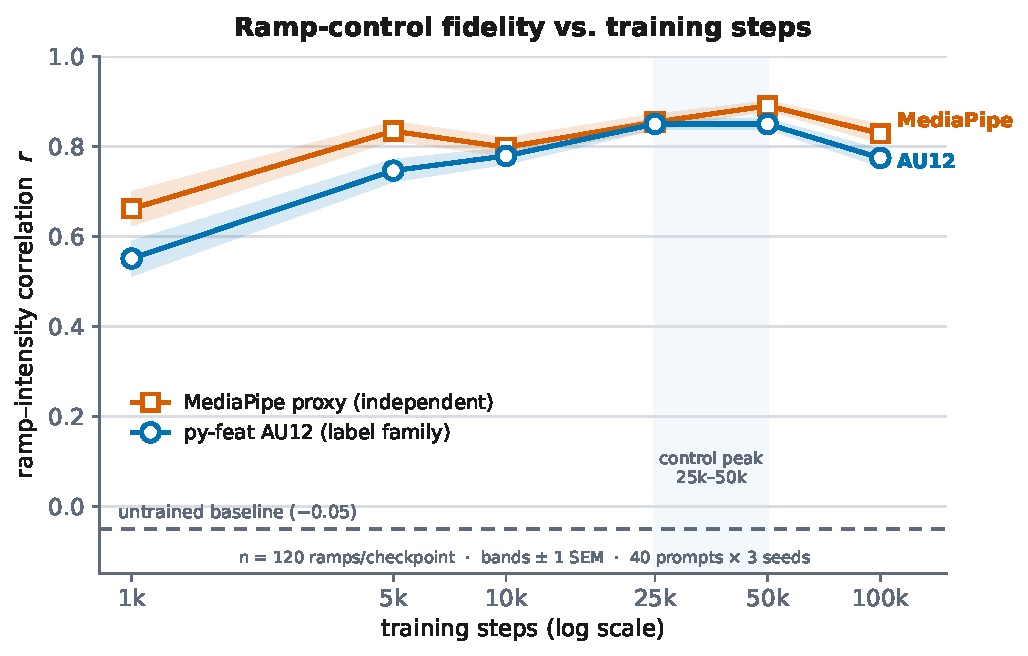
\includegraphics[width=0.78\textwidth]{images/2026-08-11-dose-response.pdf}
    \caption{Ramp-control fidelity against training steps, at six checkpoints of the single
    training run ($n=120$ ramps per checkpoint, bands $\pm1$ SEM). Both the py-feat AU12
    correlation and the label-independent MediaPipe proxy rise and plateau. Lab note 2026-08-11.}
    \label{fig:dose}
\end{figure}

A caveat follows from the curve: the released 100k checkpoint is mildly past-peak for ramp
following ($r=0.774$ against $0.850$ at 50k; Welch $t\approx3.4$), and every headline number
in this chapter comes from it. Re-evaluating at a 25k--50k checkpoint is therefore a cheap
improvement, noted as proposed work in Chapter~\ref{cap:schedule}.

% =====================================================================
\section{Comparison with the Closest Prior Art}\label{sec:res-headtohead}

% The single most important external comparison in the proposal
% (lab note 2026-07-21, n=120 matched prompts). The verdict is mixed and
% must be presented as mixed.

\begin{table}[H]
    \centering
    \caption{Head-to-head against \citet{varanka2024fineface} under matched prompts and intensity levels ($n=120$). Higher is better in every column.}
    \label{tab:res-headtohead}
    \begin{tabular}{@{}lccc@{}}
        \toprule
        System & Ramp $r$ (py-feat) & Calibration (\gls{cls}) & Identity (adjacent min.) \\
        \midrule
        FineFace, independent stills & $0.786$ & $0.50$ & baseline \\
        This work, one clip          & $0.774$ & $0.07$ & $+0.12$ \\
        \bottomrule
    \end{tabular}\\[4pt]
    {\footnotesize Source: prepared by the author. Lab note 2026-07-21.}
\end{table}

% Read the table out loud in the text, in this order:
%   1. Ramp following is a TIE (FineFace marginally ahead, and further ahead
%      on the MediaPipe proxy: 0.88 vs 0.83).
%   2. FineFace WINS absolute calibration decisively.
%   3. This work wins cross-frame identity, modestly but consistently
%      (63--68% of prompts, roughly 2.5x lower variance).
% Therefore the defensible contribution is the sequence-native formulation
% and the measurement protocol, NOT superior expression control. State this
% conclusion explicitly here so that Cap01 and Cap06 can rely on it.

Table~\ref{tab:res-headtohead} is the single most important external comparison, and its
verdict is mixed. Read in order: first, ramp following is a tie. FineFace is marginally ahead on
py-feat ($0.786$ against $0.774$) and further ahead on the MediaPipe proxy ($0.88$ against
$0.83$), a difference within noise. Second, FineFace wins absolute calibration decisively
($\gls{cls}=0.50$ against $0.07$), consistent with the ramp-only limitation of
Section~\ref{sec:res-calibration}. Third, this work wins cross-frame identity, modestly but
consistently: the adjacent-frame minimum is higher on $63$--$68\%$ of prompts, with roughly
$2.5\times$ lower variance. The conclusion, which Chapters~\ref{cap:introduction}
and~\ref{cap:schedule} rely on, is therefore explicit: the defensible contribution is the
sequence-native formulation and the measurement protocol, not superior expression control.

% =====================================================================
\section{Whole-Face Response}\label{sec:res-coactivation}

A single scalar axis invites the question of what \emph{else} it moves. Re-scoring the
ascending-ramp clips for all twenty py-feat action units, cross-checked against an
independent estimator (LibreFace) and against face-mesh geometry, shows that the axis drives
a coherent smile expression rather than an isolated muscle (Figure~\ref{fig:coactivation}).
The commanded AU12 and the Duchenne cheek raiser AU6 co-activate strongly and are
model-induced (both Spearman $r>0.87$, and significant at $q<0.05$ against the frozen
baseline); mouth-opening units (AU25/26) rise while mouth-closing and frowning units (AU23,
AU17, AU15) fall. Brow units sit near zero on py-feat, although the independent detectors
reveal a subtle brow entanglement that py-feat underreports, and the cross-check exposes one
py-feat artefact (AU20, which the independent estimator contradicts). This is a feature and a
limitation at once: the rendered change is a natural, coherent expression, but AU12 is not
isolable. It is the empirical basis for the multi-AU extension proposed in
Chapter~\ref{cap:schedule}.

\begin{figure}[t]
    \centering
    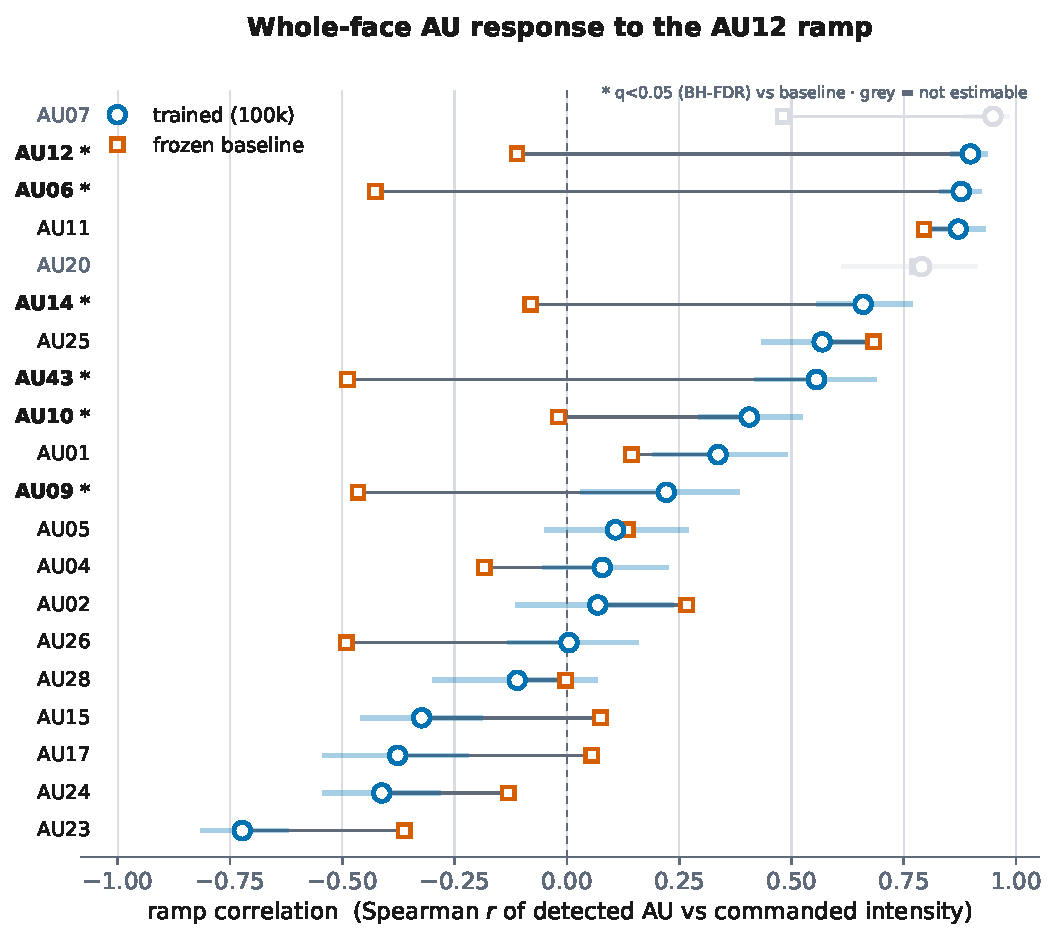
\includegraphics[width=0.72\textwidth]{images/2026-08-25-au-coactivation-profile.pdf}
    \caption{Per-action-unit response to the AU12 ramp (Spearman $r$, trained adaptor versus
    frozen baseline). The smile cluster (AU12, AU6, AU25) co-activates and the mouth-closing
    units (AU23, AU17) anti-correlate, while brow units are near zero. Asterisks mark units
    significantly modulated by training ($q<0.05$, Benjamini--Hochberg). Lab note 2026-08-25.}
    \label{fig:coactivation}
\end{figure}

% =====================================================================
\section{Qualitative Results}\label{sec:res-qualitative}

% Suggested figures (place the exported frames under images/):
%   1. One ramp: frames at commanded 0.0 to 1.0, trained vs frozen baseline.
%   2. Side-by-side with FineFace stills at matched levels, to make the
%      identity drift visible rather than merely tabulated.
%   3. A failure case. Include one; it buys credibility.

Figure~\ref{fig:qualitative} shows one ascending ramp for a single prompt and seed, with the
trained adaptor above and the frozen backbone below. With the adaptor, the commanded intensity
drives a smile that intensifies across the clip while identity and framing stay consistent;
without it, the same commanded trajectory leaves the generated portrait essentially unchanged.
The trained row also makes visible the domain shift noted in Section~\ref{sec:res-threats}: the
adaptor pulls the output toward the lab-recorded \gls{mead} appearance it was trained on.

\begin{figure}[t]
    \centering
    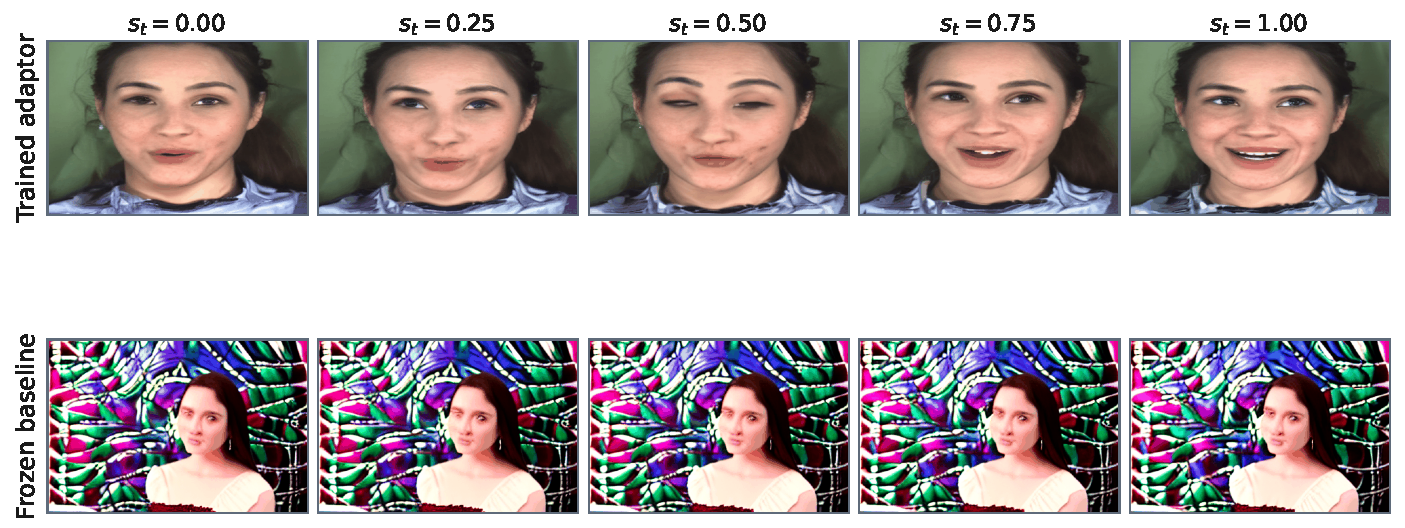
\includegraphics[width=\textwidth]{images/2026-08-25-qualitative-ramp.pdf}
    \caption{One ascending ramp (prompt: ``a portrait photograph of a young woman, frontal
    view, neutral background''; seed 42), with commanded intensity $s_t$ increasing left to
    right. Top: the trained adaptor, where the smile intensifies while identity is preserved
    across frames. Bottom: the frozen backbone under the same seed, left unchanged by the
    commanded trajectory.}
    \label{fig:qualitative}
\end{figure}

% =====================================================================
\section{Threats to Validity}\label{sec:res-threats}

\begin{itemize}
    \item \textbf{Label--evaluation circularity.} py-feat provides both the training labels and the primary metric. Mitigated by the independent MediaPipe measurement (Section~\ref{subsec:eval-circularity}), which agreed, but not eliminated.
    \item \textbf{Demographic bias.} Ramp $r$ is $0.83$ for female prompts against $0.71$ for male prompts. The prior art shows the opposite skew (FineFace: $0.82$ male against $0.77$ female), which localises the cause to the \gls{mead} training distribution rather than to AU-conditioned generation in general.
    \item \textbf{Lab-domain training data.} A single dataset, a single emotion category, frontal views, controlled lighting. Generalisation to in-the-wild portraits is untested.
    \item \textbf{Single control axis.} Only AU12 is conditioned. The whole-face analysis (Section~\ref{sec:res-coactivation}) shows the axis co-activates the entire smile cluster and cannot isolate a single unit; the prior art controls twelve action units and their combinations. A multi-AU axis is proposed in Chapter~\ref{cap:schedule}.
    \item \textbf{Single training run.} One seed, one checkpoint; no variance estimate over training runs.
\end{itemize}

\cleardoublepage
% ---------------------------------------------------------------------
\chapter{Schedule and Final Remarks}\label{cap:schedule}
\glsresetall

% =====================================================================
% SKELETON. Target: 5--8 pages.
%
% This is the chapter the banca reads most carefully in a proposal, because
% it is where they judge whether the remaining work is feasible in the time
% left. Two rules:
%   1. Every item in "remaining work" must map to a row in the timetable.
%   2. Distinguish work that needs RETRAINING (expensive, schedule it early)
%      from work that only needs inference and scoring (cheap, parallelisable).
%
% Sources: the Readiness and Evaluation Robustness checklists in
% docs/status.md. Keep this chapter in sync with them; they are the same
% list seen from two angles.
% =====================================================================

% =====================================================================
\section{Work Completed}\label{sec:sched-completed}

% Short and factual, in the order of Cap05. Resist re-arguing the results
% here; a compact list plus cross-references to Chapter~\ref{cap:preliminary-results}
% is enough.

\begin{itemize}
    \item Expression conditioning pipeline: dataset, per-frame \gls{au} supervision, embedding, training and inference entry points.
    \item Full training run to 100k steps on a single GPU.
    \item Trajectory-following evaluation at scale, with an independent estimator (Section~\ref{sec:res-ramp}).
    \item Identity-consistency measurement against a provably fair frozen-backbone baseline (Section~\ref{sec:res-identity}).
    \item Absolute-calibration measurement, with a negative outcome and a diagnosis (Section~\ref{sec:res-calibration}).
    \item Head-to-head comparison against the closest prior art under matched prompts (Section~\ref{sec:res-headtohead}).
\end{itemize}

% =====================================================================
\section{Remaining Work}\label{sec:sched-remaining}

\subsection{Requires Retraining}\label{subsec:sched-retrain}

% Schedule these first; they gate everything downstream.

\begin{itemize}
    \item \textbf{Calibration remedies.} Augment training with constant and permuted intensity trajectories so the model observes non-ramp targets; add \gls{au} dropout with \gls{cfg} on the expression condition \citep{wei2025magicface}; apply label distribution smoothing \citep{varanka2024fineface}. Target: turn the relative control of Section~\ref{sec:res-calibration} into absolute control. \todo[inline]{Decide with the advisor whether this is in scope for the dissertation or is stated as a limitation.}
    \item \textbf{Multi-AU extension.} Generalise the single AU12 axis to an AU vector, matching the control breadth of the prior art. \todo[inline]{Scope decision needed: this may be one axis too many for the time available.}
\end{itemize}

\subsection{Inference and Evaluation Only}\label{subsec:sched-eval}

% Cheap, independent, and each closes a specific checklist item.

\begin{itemize}
    \item \textbf{Training-step dose--response.} Evaluate trajectory following at intermediate checkpoints, giving independent evidence that training produces the capability. \todo[inline]{Run before any checkpoint housekeeping; the intermediate checkpoints are the raw material.}
    \item \textbf{Prompt-engineering baseline.} Graded textual smile descriptions on the unmodified backbone, answering the zero-shot objection of \citet{hua2026pixelsmile}.
    \item \textbf{Out-of-range intensity probe.} Commanded values below zero and above one, as a disentanglement check.
    \item \textbf{Multi-model identity averaging.} Add ArcFace \citep{deng2019arcface} to the existing embedding model to remove single-estimator dependence.
    \item \textbf{Perceptual and prompt-fidelity metrics.} \gls{lpips} \citep{zhang2018lpips} and CLIP-based prompt adherence on the generated clips.
\end{itemize}

\subsection{Writing}\label{subsec:sched-writing}

\todo[inline]{Dissertation chapters, and any paper submission targeted along the way.}

% =====================================================================
\section{Timetable}\label{sec:sched-timetable}

% Fill in real periods. NOTE: the date currently set in Identificacao.tex is
% 29 June 2026, which is in the past; fix it to the actual defence date
% before generating the cover (see NOTES.md).
%
% Marks: X = planned. Add or remove columns to match the real calendar.

\begin{table}[H]
    \centering
    \caption{Planned schedule for the remaining work.}
    \label{tab:timetable}
    \footnotesize
    \begin{tabular}{@{}lcccccc@{}}
        \toprule
        Activity & \multicolumn{6}{c}{Two-month period} \\
        \cmidrule(l){2-7}
                 & 1 & 2 & 3 & 4 & 5 & 6 \\
        \midrule
        Calibration remedies (retraining)   & X & X &   &   &   &   \\
        Training-step dose--response         & X &   &   &   &   &   \\
        Prompt-engineering baseline          & X &   &   &   &   &   \\
        Out-of-range intensity probe         &   & X &   &   &   &   \\
        Multi-model identity averaging       &   & X &   &   &   &   \\
        Perceptual / prompt-fidelity metrics &   & X & X &   &   &   \\
        Multi-AU extension (if in scope)     &   &   & X & X &   &   \\
        Consolidated final evaluation        &   &   &   & X & X &   \\
        Dissertation writing                 & X & X & X & X & X & X \\
        Revision and defence                 &   &   &   &   & X & X \\
        \bottomrule
    \end{tabular}\\[4pt]
    {\footnotesize Source: prepared by the author.}
\end{table}

\todo[inline]{Replace the generic periods with real months and confirm the defence deadline with the advisor.}

% =====================================================================
\section{Risks and Mitigations}\label{sec:sched-risks}

% State these proactively. A proposal that names its own risks reads as
% better planned than one the banca has to interrogate.

\begin{itemize}
    \item \textbf{The calibration remedies may not work.} Mitigation: the sequence-native formulation and the measurement protocol stand as contributions independently of whether absolute calibration is achieved; the negative result is itself reportable and diagnosed.
    \item \textbf{Scope creep across control axes.} Mitigation: treat the multi-AU extension as optional and decide by a fixed date.
    \item \textbf{Single-dataset generalisation.} Mitigation: state the lab-domain restriction as a scope boundary rather than attempting a new dataset late in the schedule.
    \item \textbf{Compute limits.} A single consumer GPU against prior art trained on multi-GPU clusters. Mitigation: the frozen-backbone design keeps trainable parameters small; report compute honestly as a constraint of the setup.
\end{itemize}

% =====================================================================
\section{Final Remarks}\label{sec:sched-final}

% Close on what the work will have established, phrased consistently with
% Section~\ref{sec:res-headtohead}: the contribution is the sequence-native
% formulation of expression intensity plus the measurement protocol, not a
% claim of superior expression control. Keep this consistent with Cap01;
% the two chapters are read together.

\todo[inline]{Two or three paragraphs. Write last, and check it agrees with Cap01 word for word on the contribution claim.}

\cleardoublepage

% =====================================================================
% Bibliography
% =====================================================================
\markright{Bibliography}
\bibliographystyle{apalike}
%\bibliographystyle{ieeetr}
{
	\addcontentsline{toc}{chapter}{Bibliography}
	\bibliography{Ref/references}
}
\cleardoublepage

\end{document}
